\documentclass{beamer}

\title{An argumentation based solution to making schedules}
\author{Pim van der Meulen \and Ren\'e Mellema \and Xeryus Stokkel}
\date{October 24, 2016}

\usetheme{Luebeck}

\begin{document}

\frame{\titlepage}

\section{Introduction}
\begin{frame}
	\frametitle{Introduction}
	
\includegraphics[width=0.52\textwidth]{Schedule.jpg}%
	
\includegraphics[width=0.48\textwidth]{Argument.jpg}
\end{frame}

\section{State of the art}
\begin{frame}
	\frametitle{Syllabus Plus}
	\begin{columns}%[c] % the "c" option specifies center vertical alignment
    \column{.8\textwidth} % column designated by a command
    \begin{enumerate}
		\item Used by colleges and universities all over the world, including the University of Groningen
		\item Constraint satisfaction problem solver:
		\begin{enumerate}
			\item Constraints
			\item Rules
			\item Preferences
		\end{enumerate}
	\end{enumerate}
    \column{.2\textwidth}
    
\includegraphics[width=\textwidth]{SyllabusPlus.png}
    \end{columns}	
\end{frame}

\section{Our approach}
\subsection{Argumentation Framework}
\begin{frame}
    \frametitle{Argumentation Framework}
    \begin{columns}
        \column{.6\textwidth}
        \begin{itemize}
            \item Argument relations:
                \begin{itemize}
                    \item Attack
                    \item Support
                    \item Undercut
                \end{itemize}
            \item Groundedness:
                \begin{itemize}
                    \item No attacks
                    \item More support than attack
                \end{itemize}
        \end{itemize}
        \column{.4\textwidth}
        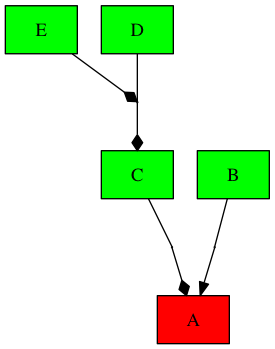
\includegraphics[width=\textwidth]{framework.png}
    \end{columns}
\end{frame}

\subsection{Scheduling}
\begin{frame}
	\frametitle{Our approach}
        \begin{itemize}
            \item Go over all available rooms and times
            \item Agents (``Lecturers'') make claim if course fit
            \item Agents support their arguments, undercut others
            \item Continues until no new arguments are made
            \item Claim that is grounded at the end wins
        \end{itemize}
\end{frame}

\subsection{Types of arguments to use}
\begin{frame}
	\frametitle{Argument types}
	\begin{enumerate}
		\item Size argument 
		\item Beamer argument
		\item Preference argument
	\end{enumerate}
\end{frame}

\subsection{Data input}
\begin{frame}
	\frametitle{Data input}
	\center{}
	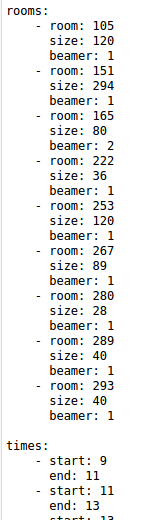
\includegraphics[width=0.2\textwidth]{Rooms.png}%
	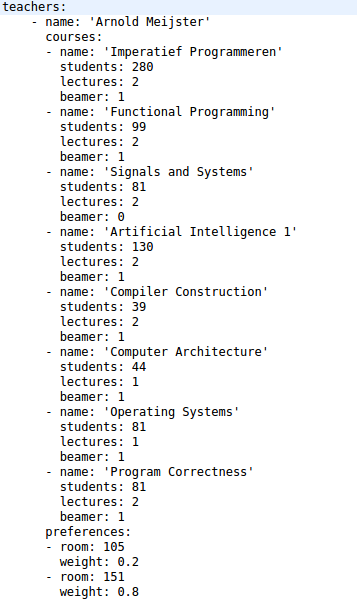
\includegraphics[width=0.365\textwidth]{Teachers.png}
\end{frame}

\section{Results}
\begin{frame}
	\frametitle{Results}
\end{frame}

\section{Relevance}
\begin{frame}
	\frametitle{Relevance}
        \begin{itemize}[<+->]
            \item Generalized for resource negotiation in MAS
            \item Extract reasons for room allocation
        \end{itemize}
\end{frame}

\frame{\frametitle{Questions?}}

\end{document}
